

\section{Internet infrastructure}

\begin{theorem}
    {Moore's Law}
    The number of transistors on an integrated circuit doubles about every two years.
\end{theorem}

\subsection{Extranet vs Intranet}

\begin{itemize}
    \item \textbf{Extranet}: A network that is connected to the internet.
    \item \textbf{Intranet}: A network that is not connected to the internet.
\end{itemize}

\subsection{Architecture}

\begin{definition}
    {ISP}
    The global internet is connected by fiber optic cables, with \textbf{Internet Service Providers (ISP)} connecting devices to the internet. The optic cables are prone to natural hazards as well as human activities like ship anchoring.
\end{definition}

\begin{definition}
    {NAP}
    The ISPs connect to the internet through \textbf{Network Access Points (NAP)}. They are high speed routers that connect to the internet.
\end{definition}

\subsection{Speed}

\begin{definition}
    {Bandwidth}
    The amount of data that can be transmitted through a network per unit of time.
\end{definition}

\subsection{Network protocols}

\begin{definition}
    {Protocol}
    A format for transmitting packets (data) that has been agreed by a standard organization or industry.

    \textbf{IP}: Internet Protocol

    \textbf{TCP}: Transmission Control Protocol
\end{definition}

\begin{theorem}
    {Packet switching}
    \begin{enumerate}
        \item The data is divided into packets.
        \item Each packet is transmitted to the destination through the network by different paths.
        \item The destination is responsible for reassembling the packets into the original data.
    \end{enumerate}
    \begin{itemize}
        \item \textbf{TCP}: Ordering packets\\
              Forming packets (adding headers and control information), dividing and reassembling, collision control (error checking)
        \item \textbf{IP}: Routing packets\\
              Send to proper destination, addresses
    \end{itemize}
\end{theorem}

\subsection{IP Addresses}

\begin{definition}
    {IP Address}
    A unique identifier for a device on the internet. Generic form called \textbf{IPv4}.

    x.x.x.x where x is a number between 0 and 255.
\end{definition}

\begin{theorem}
    {Dynamic IP addresses}
    When device connected to internet, it is assigned a temporary IP address. When the connection is lost, the IP address is released and assigned to another device.
\end{theorem}

\begin{definition}
    {Domain Name}
    A human-readable name for an IP address.
\end{definition}

\begin{definition}
    {Domain Name System (DNS)}
    A distributed database that translates domain names to IP addresses. It is stored by your \textbf{ISPs}.
\end{definition}

\begin{figure}[h!]
    \centering
    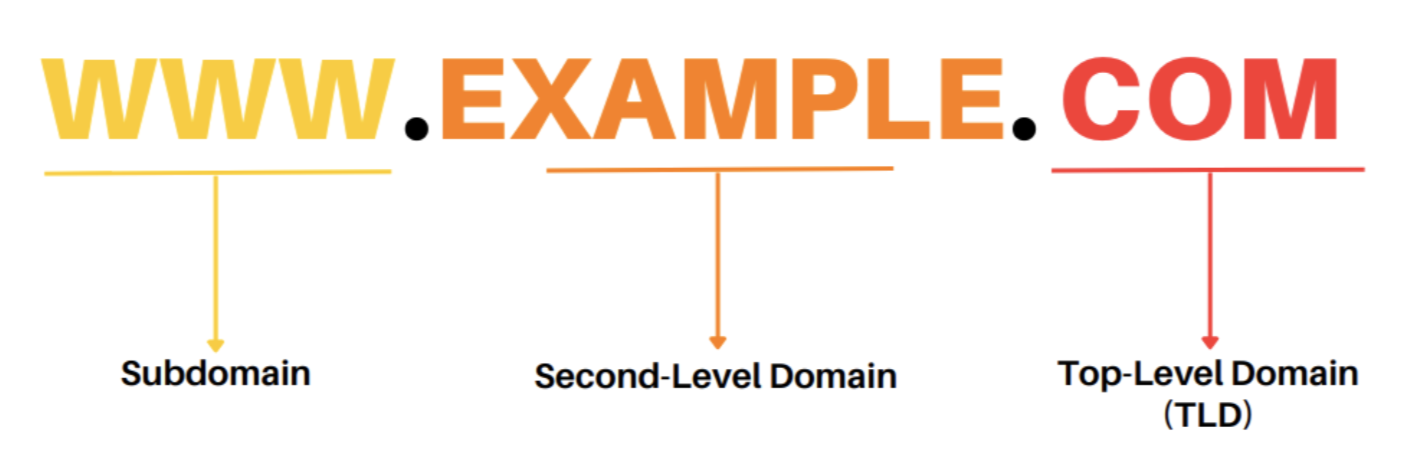
\includegraphics[width=0.8\textwidth]{images/tld.png}
    \caption{Structure of Domains Names}
    \label{fig:tld_structure}
\end{figure}

\subsection{Open source software}

\begin{definition}
    {Open source software (OSS)}
    Software that is free to use, modify, and distribute.
    \begin{itemize}
        \item \textbf{Free}: Free of charge
        \item \textbf{Source code}: Available for public inspection
        \item \textbf{Licensed}: Original author retains copyright and terms of use.
        \item \textbf{Repository}: Code is usually shared on \textbf{GitHub}, users can freely download, use, modify, and distribute.
    \end{itemize}
\end{definition}

There are a few problems that comes with open source software:

\begin{itemize}
    \item \textbf{Support}: There is no guarantee of support from the original author.
    \item \textbf{Administration}: Malware and viruses can be introduced unintentionally.
    \item \textbf{Quality assurance}: Quality of contribution is not guaranteed.
    \item \textbf{Legal issues}: Legal disputes may arise from patent infringement.
    \item \textbf{Security}: Security vulnerabilities may exist in the software.
\end{itemize}

\begin{definition}
    {Total cost of ownership (TCO)}
    The total cost of owning a software system beyond the purchase price. This includes costs like \textbf{maintenance}, \textbf{upgrades}, \textbf{service}, and \textbf{support}.

    For OSS, the TCO is usually lower than that of proprietary software, as the cost of support is distributed among the users.
\end{definition}

\begin{definition}
    {LAMP stack}
    The usage of 4 OSS to build a web service, powering services such as Youtube.
    \begin{itemize}
        \item \textbf{Linux}: Operating system
        \item \textbf{Apache}: Web server
        \item \textbf{MySQL}: Database
        \item \textbf{PHP}: Programming language
    \end{itemize}
\end{definition}

\subsection{Cloud computing}

\begin{definition}
    {Cloud computing}
    Data sent to shared computing resources over the internet, and sent back when completed.
\end{definition}

\begin{theorem}
    {Cloud computing models}
    \begin{itemize}
        \item \textbf{Infrastructure as a Service (IaaS)}: Provides virtualized computing resources over the internet.
        \item \textbf{Platform as a Service (PaaS)}: Provides a platform for developing and deploying applications.
        \item \textbf{Software as a Service (SaaS)}: Provides software applications that are accessed over the internet.
    \end{itemize}
\end{theorem}

Potential problems of cloud computing:

\begin{itemize}
    \item \textbf{Data privacy}: Data may be leaked to other users.
    \item \textbf{Service availability}: Service may be unavailable.
    \item \textbf{Vendor lock-in}: Switching to another vendor is difficult as the data is usually held by the vendor.
\end{itemize}

\subsection{Internet of things (IoT)}
\begin{definition}
    {Internet of things (IoT)}
    A network of physical devices that can connect and exchange data over a network without requiring human-to-computer interaction. It consists of 3 layers:
    \begin{itemize}
        \item \textbf{Perception layer}: Interact with the physical environment, like Sensors \& actuators
        \item \textbf{Network layer}: Discovers, connects \& translates the perception layer to the application layer
        \item \textbf{Application layer}: Store \& process data
    \end{itemize}
\end{definition}
